\newpage
\section{Introduction REPTAR}
\subsection{Mise en place de l'environnement, utilisation de git}
\textbf{a) Donnée: }Il faut tout d'abord récupérer le dépôt étudiant pour les laboratoires SEEE à l'aide de la commande
suivante (via une fenêtre de terminal):
\begin{lstlisting}
$ git clone firstname.lastname@eigit.heig-vd.ch:/home2/reds/seee/seee_student
\end{lstlisting}

\textbf{Travail réalisé: }
Nous n'avions pas les droits d'accès pour le dépôt git, nous l'avons donc téléchargé, puis extrait depuis le lien:
\url{https://drive.switch.ch/index.php/s/TbHxQZtmO9IVdkb}.\\
Le dossier seee\_student a ensuite été placé dans: /home/redsuser/\\

\textbf{b) Donnée: }Lancez Eclipse et ouvrez le workspace seee\_student. Vous devriez obtenir la liste des projets (à
gauche). Chaque projet a un lien symbolique dans la racine du workspace. \\\\
\textbf{Travail réalisé: }
En introduisant le path du dossier seee\_student comme workspace au lancement d'Eclipse, nous obtenons la liste de projets suivante:
\begin{figure}[H]
	\begin{center}
		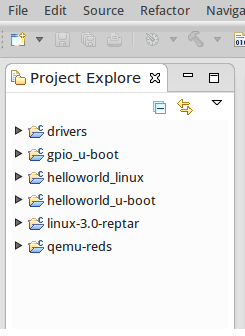
\includegraphics[height=7cm]{img/eclipseProjet.png}
		\caption{Liste des projets}
		\label{eclipseProjet}
	\end{center}
\end{figure}

\textbf{c) Donnée: }Compilez maintenant l'émulateur Qemu. Dans une fenêtre de terminal, lancez la commande
suivante à partir de votre répertoire seee\_student : 
\begin{lstlisting}
$ make qemu
\end{lstlisting}
\textbf{Travail réalisé: }
Vu que nous n'avons pas téléchargé le dossier de projets depuis git, il faut nettoyer le contenu du dossier avec clean ou distclean avant de pourvoir utiliser qemu. Le make qemu prend quelques instants.\\
\begin{lstlisting}
redsuser@vm-reds-2015s2:~/seee_student$ make clean
redsuser@vm-reds-2015s2:~/seee_student$ make qemu
...
make[1]: Leaving directory `/home/redsuser/seee_student/qemu-reds'
redsuser@vm-reds-2015s2:~/seee_student$
\end{lstlisting}

\subsection{Démarrage de Qemu}
\textbf{a) Donnée: }Depuis Eclipse, lancez le debugger avec la configuration de debug « qemu-reds Debug ». Dans la
fenêtre Console, vous pourrez entrer directement des commandes de U-boot (tapez help par
exemple). \\\\
\textbf{Travail réalisé: }
\begin{figure}[H]
	\begin{center}
		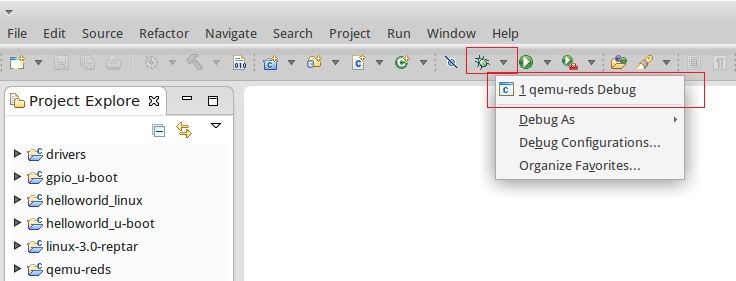
\includegraphics[height=7cm]{img/manip2Intro.png}
		\caption{Lancement d'Eclipse en mode Debug}
		\label{eclipseDebug}
	\end{center}
\end{figure}
\textbf{Remarque: }Après le lancement du Debug, il faut changer d'onglet en haut à droite en choisissant \textit{Debug} pour avoir la console. Ce changement d'onglet ne se fait pas automatiquement.
\begin{figure}[H]
	\begin{center}
		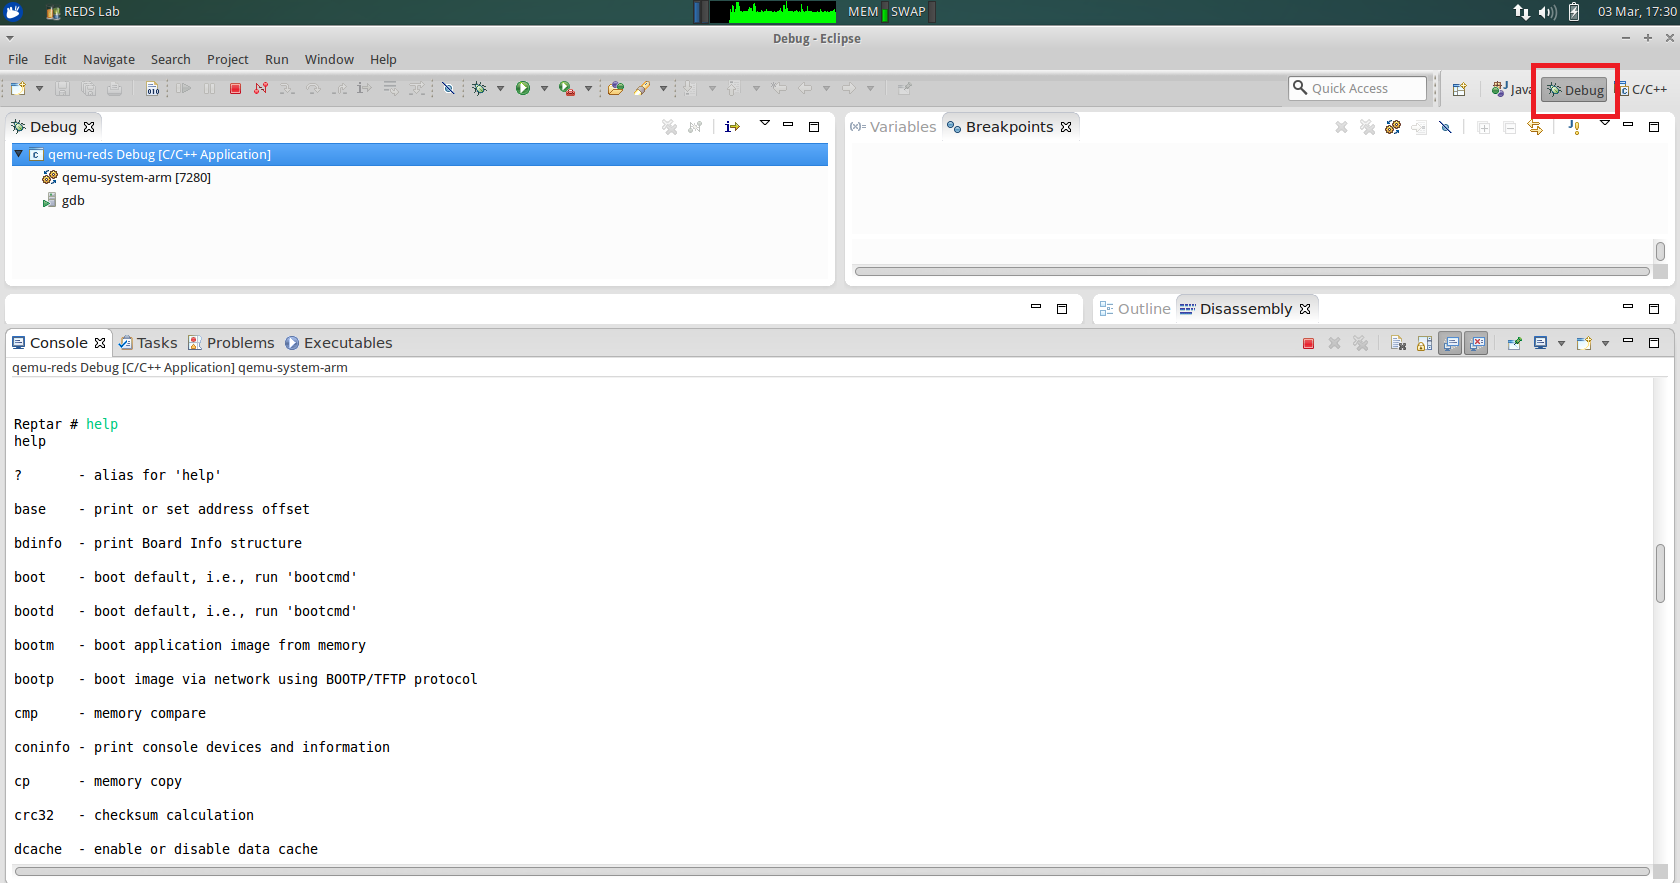
\includegraphics[width=18cm]{img/ubootCommand.png}
		\caption{Command help dans l'U-boot}
		\label{ubootCommand}
	\end{center}
\end{figure}
En interrompant le programme avec le bouton \textit{suspend}, on obtient la vue assembleur ci-dessous. L'environnement essaie d'ouvrir le fichier ppoll.c, on est donc en attente d'un événement. Le programme est interrompu après un syscall, il compare deux valeurs ce qui confirme qu'il est effectivement en attente d'événements. L'adresse comparée est sur 64bits, cela nous indique que l'on est sur l'environnement émulé de la machine hôte. Sur le Reptar, l'adresse serait 32bits.
\begin{figure}[H]
	\begin{center}
		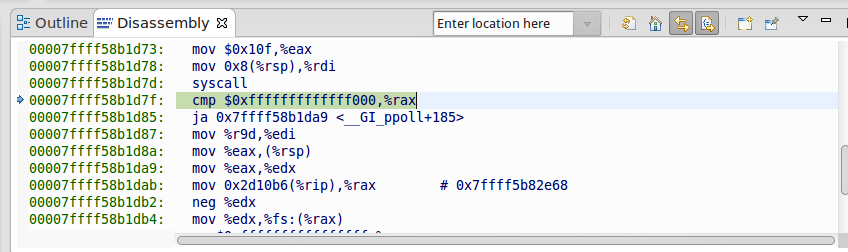
\includegraphics[width=18cm]{img/ubootAsm.png}
		\caption{Command help dans l'U-boot}
		\label{ubootAsm}
	\end{center}
\end{figure}
\textbf{c) Donnée: } Stoppez l'exécution, et dans une fenêtre de commande, démarrez qemu à l'aide du script stf (en
tapant ./stf) dans le répertoire racine. Vous arrivez dans U-boot. \\\\
\textbf{Travail réalisé: }Cette partie n'a plus rien avoir avec Eclipse, on peut le fermer et lancer un terminal.
Avec la commande \textit{stf} tapée à la racine du répertoire seee\_student, on arrive au même point qu'en lançant le Debug dans Eclipse. On peut également essayer la commande \textit{help}
\begin{lstlisting}
redsuser@vm-reds-2015s2:~/seee_student$ ./stf
WARNING: Image format was not specified for 'filesystem/flash' and probing guessed raw.
...

Reptar # help
?       - alias for 'help'
base    - print or set address offset
bdinfo  - print Board Info structure
boot    - boot default, i.e., run 'bootcmd'
bootd   - boot default, i.e., run 'bootcmd'
bootm   - boot application image from memory
bootp   - boot image via network usi
...
\end{lstlisting}

\subsection{Tests avec U-boot}
\textbf{a) Donnée: }Dans U-boot, listez les variables d'environnement avec la commande printenv. Observez les
variables prédéfinies « tftp1, tftp2 et goapp ». Ces variables définissent des commandes U-boot qui
peuvent être exécutées à l'aide de la commande run (par exemple run tftp1).
La commande go <addr> permet de lancer l'exécution à l'adresse physique <addr>.
Vous pouvez définir/modifier vos propres variables et les sauvegarder dans la flash émulée avec la
commande saveenv (seulement avec le lancement via stf). \\\\
\textbf{Travail Réalisé: }\\\\

\textbf{b) Donnée: }La production de l'exécutable helloworld\_u-boot s'effectue en tapant la commande make dans le
répertoire contenant les sources du programme. Ensuite, vous pouvez transférer le fichier (extension
.bin) dans U-boot et exécuter le binaire (aidez-vous des variables d'environnement prédéfinies). \\\\
\textbf{Travail réalisé: }\\\\

\textbf{c) Donnée: } Testez le debugger dans Eclipse avec le projet helloworld\_u-boot. Mettez un breakpoint dans le
code source au démarrage du programme, et lancez le debugger avec la configuration de debug
« helloworld\_u-boot Debug ». \\\\
\textbf{Travail Réalisé: }

\subsection{Tests avec Linux}
\textbf{a) Donnée: }Lancez le script ./deploy qui permettra de déployer le noyau Linux dans la sdcard virtuelle (ignorez
l'erreur due à l'absence de certains fichiers). \\\\
\textbf{Travail réalisé: }\\\\
\textbf{b) Donnée: }Poursuivez ensuite en cross-compilant l'application helloworld pour Linux (via make). \\\\
\textbf{Travail réalisé: }\\\\
\textbf{c) Donnée: }Copiez l'exécutable dans le rootfs\\\\
\textbf{Travail réalisé: }\\\\
\textbf{d) Donnée: }Lancez le script stq suivi de la commande boot dans U-boot pour amorcer le démarrage de Linux\\\\
\textbf{Travail réalisé: }\\\\
\textbf{e) Donnée: }Lancez votre application\\\\
\textbf{Travail réalisé: }\\\\
\textbf{f) Donnée: }Dans Linux, tapez la commande suivante :
\begin{lstlisting}
$ /usr/share/qt/examples/effects/lighting/lighting -qws & 
\end{lstlisting}
\textbf{Travail réalisé: }

\subsection{Tests sur la plate-forme réelle}
\textbf{a) Donnée: }Déployez l'application helloworld dans U-boot sur la plate-forme REPTAR avec l'interface réseau.
Le transfert peut s'effectuer avec la commande tftp.
Il est nécessaire d’exécuter la commande suivante pour mettre à jour les adresses IP et MAC de la plate-forme
REPTAR : 
\begin{lstlisting}
# run setmac setip 
\end{lstlisting}
\textbf{Travail réalisé: }\\\\
\textbf{b) Donnée: }Déployez l'application helloworld dans Linux à l'aide du réseau et de la commande scp.\\\\
\textbf{Travail réalisé: }\\\\

\subsection{Accès aux périphériques REPTAR}
\textbf{a) Donnée: } Sur la base de l’exemple gpio\_u-boot., vous devez développer une application permettant d’interagir avec les
LEDs et les switchs présents sur la carte CPU de la plate-forme REPTAR.
Le but de l’application est d’allumer une LED lorsqu’on appuie sur un switch.
\begin{enumerate}
	\item La LED 0 doit s’allumer lorsqu’on appuie sur le SWITCH 0.
	\item La LED 1 s’allume si l’on appuie sur le SWITCH 1.
	\item Et ainsi de suite pour les LEDs et switchs 0..3 de la carte CPU.
\end{enumerate}
Le switch numéro 4 sert à quitter l’application. Aidez-vous des fichiers d'en-tête (\#include) déjà présents dans
le chablon fourni.\\
L’application gpio\_u-boot est à déployer dans U-boot via la commande tftp. \\\\
\textbf{Travail réalisé: }\\\\